%%%%%%%%%%%%%%%%%%%%%%%%%%%%%%%%%%%%%%%%%%%%%%%%%%%%%%%%%%%%%%%%%%%%%%%%%%%%%%%%%%%%%%%%%%%%%%%%%%%%%%%%%%%%%%%%%%%%%%%%%%%%%%%%%%%%%%%%%%%%%%%%%%%%%%%%%%%%%%%%%%%
% Written By Michael Brodskiy
% Class: Analysis of Random Phenomena
% Professor: I. Salama
%%%%%%%%%%%%%%%%%%%%%%%%%%%%%%%%%%%%%%%%%%%%%%%%%%%%%%%%%%%%%%%%%%%%%%%%%%%%%%%%%%%%%%%%%%%%%%%%%%%%%%%%%%%%%%%%%%%%%%%%%%%%%%%%%%%%%%%%%%%%%%%%%%%%%%%%%%%%%%%%%%%

\documentclass[12pt]{article} 
\usepackage{alphalph}
\usepackage[utf8]{inputenc}
\usepackage[russian,english]{babel}
\usepackage{titling}
\usepackage{float}
\usepackage{amsmath}
\usepackage{graphicx}
\usepackage{enumitem}
\usepackage{amssymb}
\usepackage[super]{nth}
\usepackage{everysel}
\usepackage{ragged2e}
\usepackage{geometry}
\usepackage{multicol}
\usepackage{fancyhdr}
\usepackage{cancel}
\usepackage{siunitx}
\usepackage{physics}
\usepackage{tikz}
\usepackage{mathdots}
\usepackage{yhmath}
\usepackage{cancel}
\usepackage{color}
\usepackage{xcolor}
\usepackage{colortbl}
\usepackage{array}
\usepackage{multirow}
\usepackage{gensymb}
\usepackage{tabularx}
\usepackage{extarrows}
\usepackage{booktabs}
\usepackage{lastpage}
\usetikzlibrary{fadings}
\usetikzlibrary{patterns}
\usetikzlibrary{shadows.blur}
\usetikzlibrary{shapes}

\geometry{top=1.0in,bottom=1.0in,left=1.0in,right=1.0in}
\newcommand{\subtitle}[1]{%
  \posttitle{%
    \par\end{center}
    \begin{center}\large#1\end{center}
    \vskip0.5em}%

}
\usepackage{hyperref}
\hypersetup{
colorlinks=true,
linkcolor=blue,
filecolor=magenta,      
urlcolor=blue,
citecolor=blue,
}


\title{Homework 1}
\date{\today}
\author{Michael Brodskiy\\ \small Professor: I. Salama}

\begin{document}

\maketitle

\begin{enumerate}

  \item 

    \begin{enumerate}

      \item We know that union is a set containing all elements from both $A$ and $B$. Thus, we get:

        $$\boxed{A\cup B=\left\{ \bold{4\text{\textbf{GB}},8\text{\textbf{GB}},12\text{\textbf{GB}},32\text{\textbf{GB}}} \right\}}$$

        On the other hand, an intersection is all elements common to $A$ and $B$. Thus, we get:

        $$\boxed{A\cap B=\left\{ \bold{32\text{\textbf{GB}}} \right\}}$$

      \item Complements contain all elements from the sample space, less the elements present in the original set, thus, we get:

        $$\boxed{A^c=\left\{ \bold{4}\text{\textbf{GB}}, \bold{12}\text{\textbf{GB}}, \bold{16}\text{\textbf{GB}}, \bold{64}\text{\textbf{GB}} \right\}}$$
        $$\boxed{B^c=\left\{ \bold{8}\text{\textbf{GB}}, \bold{16}\text{\textbf{GB}}, \bold{64}\text{\textbf{GB}} \right\}}$$

      \item Set subtraction removes elements common to both sets. Thus, we get:

        $$\boxed{B-A=\left\{ \bold{4}\text{\textbf{GB}},\bold{12}\text{\textbf{GB}} \right\}}$$

        $A$ and $B^c$ from above, we take the intersection to find:

        $$\boxed{A\cap B^c=\left\{ \bold{8}\text{\textbf{GB}}\right\}}$$

      \item We know that $B\cap A= A\cap B$, and, therefore, we perform the following operation:

        $$\left\{ \bold{4}\text{\textbf{GB}},\bold{12}\text{\textbf{GB}} \right\}\cup \left\{ \bold{32\text{\textbf{GB}}} \right\}$$

        This gives us:

        $$\boxed{(B-A)\cup (B\cap A)=\left\{ \bold{4}\text{\textbf{GB}},\bold{12}\text{\textbf{GB}}, \bold{32}\text{\textbf{GB}} \right\}}$$

        We can note that this simply returns our original $B$.

      \item First, we find the complement of the union. From (a) we take the complement of the union to get:

        $$\boxed{(A\cup B)^c=\left\{ \bold{16}\text{\textbf{GB}},\bold{64}\text{\textbf{GB}} \right\}}$$

        Alternatively, we find the intersection of the $A$ and $B$ complements from part (b) to see:

        $$\boxed{A^c\cap B^c=\left\{ \bold{16}\text{\textbf{GB}},\bold{64}\text{\textbf{GB}} \right\}}$$

        As De Morgan's Laws state, the two should be equivalent.

    \end{enumerate}

  \item 

    \begin{enumerate}

      \item The sample space is made up of permutations of the possible modes for three processors. This gives us:

        $$\boxed{S=\left\{ \text{\textbf{AAA}},\text{\textbf{AAB}},\text{\textbf{ABA}},\text{\textbf{ABB}},\text{\textbf{BAA}},\text{\textbf{BAB}},\text{\textbf{BBA}},\text{\textbf{BBB}} \right\}}$$

        Note that we may confirm that this is an exhaustive list, as there are 3 binary options meaning that there are $2^3=8$ possible permutations of these modes, as shown above.

      \item Event 1 constrains the sample space to all cases in which the first processor operates in \textbf{Mode} `\textbf{A}' which gives us:

        $$\boxed{\bold{E_1}=\left\{ \text{\textbf{AAA}},\text{\textbf{AAB}},\text{\textbf{ABA}},\text{\textbf{ABB}} \right\}}$$

      \item Event 2 constrains the sample space to all cases in which the first and third processors operate in \textbf{Mode} `\textbf{B}' which gives us:

        $$\boxed{\bold{E_2}=\left\{ \text{\textbf{BAB}},\text{\textbf{BBB}}\right\}}$$

      \item We can take the intersection of the two events to find:

        $$\bold{E_1}\cap\bold{E_2}=\emptyset$$

        \underline{Therefore, the two are mutually exclusive}

      \item Taking the union of the two events, we find:

        $$\bold{E_1}\cap\bold{E_2}\neq S$$

        \underline{Therefore, the two are \textbf{not} collectively exhaustive}

      \item Subtracting $\bold{E_2}$ from $\bold{E_1}$ gives us:

        $$\bold{E_1}-\bold{E_2}$$

        Given that the two share no elements, we simply get $\bold{E_1}$ such that:

        $$\bold{E_1}-\bold{E_2}=\bold{E_1}=\left\{ \text{\textbf{AAA}},\text{\textbf{AAB}},\text{\textbf{ABA}},\text{\textbf{ABB}} \right\}$$

    \end{enumerate}

    \setcounter{enumi}{3}

  \item We can express the event $A$ as:

    $$A=\left\{ (i,j)\,\Big|\,|i-j|=1,\, i+j>4 \right\}$$

    First, let us define pairs such that $|i-j|=1$. This gives us:

    $$E_{|i-j|=1}=\left\{(1,0),(1,2),(3,2),(3,4)  \right\}$$

    Then, we define pairs such that $i+j>4$:

    $$E_{i+j>4}=\left\{(3,2),(3,4),(4,2),(4,4)  \right\}$$

    We then take the intersection of the two sets to find:

    $$\boxed{A=\left\{ (3,4),(3,2) \right\}}$$

    We know that the total amount of outcomes (since each is equally likely) is the quantity of possibilities of $i$ time the quantity of possibilities of $j$, which gives us the quantity of elements in $S$:

    $$N_S=(3)(4)=12$$

    Given that there are two outcomes possible for $A$, we can find the probability of $A$ occurring as:

    $$\boxed{P[A]=\frac{2}{12}=.1667}$$

  \item 

    \begin{enumerate}

      \item First and foremost, we may rewrite $P[A\cup B]$ to get:

        $$P[A]+P[B]-P[A\cap B]\geq P[A]$$

        This is equivalent to:

        $$P[A]+P[A^c\cap B]\geq P[A]$$

        Subtracting over, we get:

        $$P[A^c\cap B]\geq 0$$

        Since probability must always be greater than or equal to zero, we know that the above statement will always be true, and, therefore, the following must be true as well:

        $$\boxed{\therefore P[A\cup B]\geq P[A]}$$

      \item Similarly to part $A$, we may rewrite $P[A\cap B]$ to get:

        $$P[A]+P[B]-P[A\cup B]\leq P[A]$$

        We subtract over to get:

        $$P[B]-P[A\cup B]\leq 0$$
        $$P[B]\leq P[A\cup B]$$

        Since a union will always have either more or an equal amount of elements as the original set, the above statement is always true, and, therefore, we may write:

        $$\boxed{\therefore P[A\cap B]\leq P[A]}$$

      \item Since subtraction removes common elements, we know that there may be two cases: $A$ and $B$ have common elements, or $A$ and $B$ have no common elements. In the case of the latter, we know that the two are mutually exclusive, and therefore: $P[A-B]=P[A]-P[B]$, which gives us:

        $$P[A]-P[B]\leq P[A]$$
        $$P[B]\geq0$$

        We know that the above statement is always true, since probability can not be negative. Now, in the case of the former, set $A-B$ would contain less elements than $A$. Therefore, we can state that:

        $$\boxed{\therefore P[A-B]\leq P[A]}$$

    \end{enumerate}

  \item 

    \begin{enumerate}

      \item The first event (among $A,B,$ and $C$ only $B$ is applied) is shown below:

        \begin{figure}[H]
          \centering
          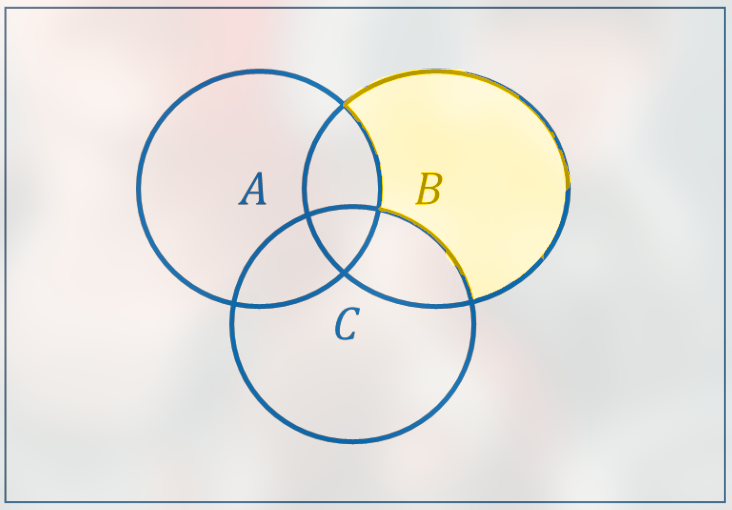
\includegraphics[width=.7\textwidth]{Figures/HW1-6a}
          \caption{Event 1 Highlighted in Gold}
          \label{fig:1}
        \end{figure}

        This set can be expressed as:

        $$\boxed{\bold{E_1}=B- (A\cup C)}$$

      \item The second event (at least one technique, $A$, $B$, or $C$ is applied) is shown below:

        \begin{figure}[H]
          \centering
          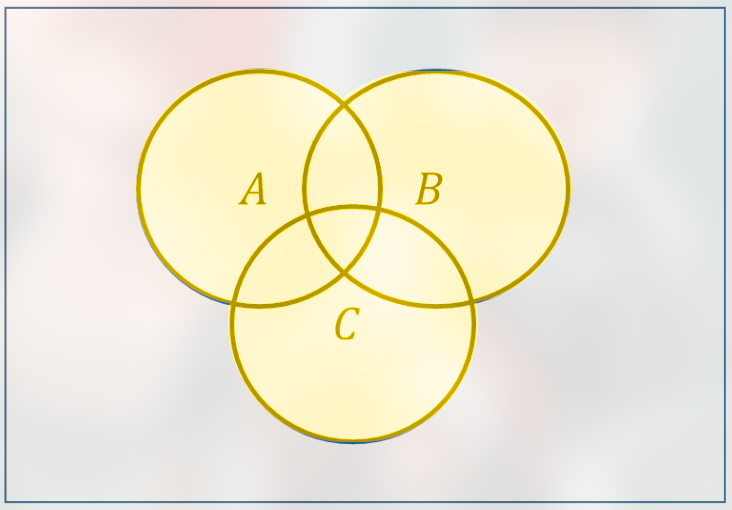
\includegraphics[width=.7\textwidth]{Figures/HW1-6b}
          \caption{Event 2 Highlighted in Gold}
          \label{fig:2}
        \end{figure}

        This set can be expressed as:

        $$\boxed{\bold{E_2}=A\cup B\cup C}$$

      \item The third event ($A$ and $C$, but not $B$ are applied) is shown below:

        \begin{figure}[H]
          \centering
          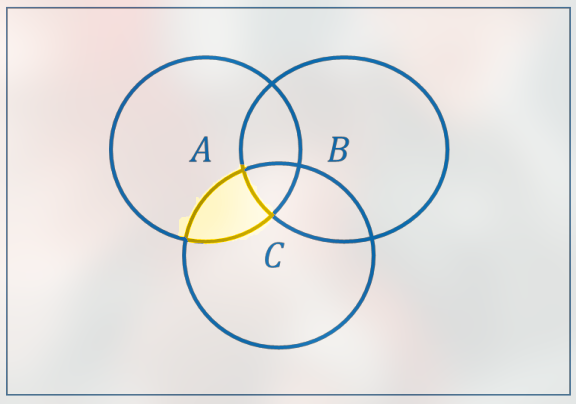
\includegraphics[width=.7\textwidth]{Figures/HW1-6c}
          \caption{Event 3 Highlighted in Gold}
          \label{fig:3}
        \end{figure}

        This can be expressed as:

        $$\boxed{\bold{E_3}=A\cap C - B}$$

      \item The fourth event (at most two of the techniques are applied) is shown below:

        \begin{figure}[H]
          \centering
          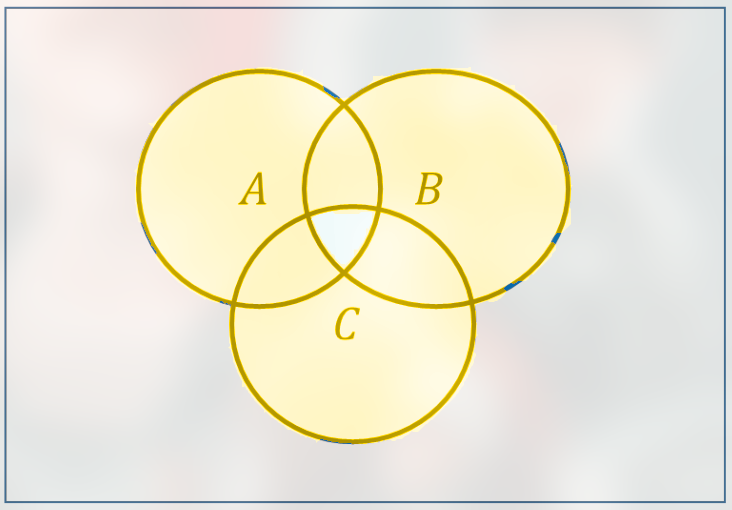
\includegraphics[width=.7\textwidth]{Figures/HW1-6d}
          \caption{Event 4}
          \label{fig:4}
        \end{figure}

        This can be expressed as:

        $$\boxed{\bold{E_4}=(A\cup B\cup C)- (A\cap B\cap C)}$$

      \item The fifth event (only one technique is applied) is shown below:

        \begin{figure}[H]
          \centering
          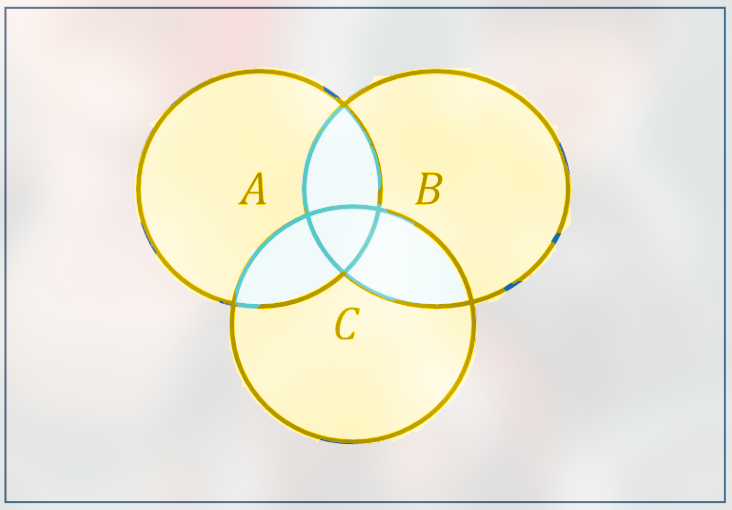
\includegraphics[width=.7\textwidth]{Figures/HW1-6e}
          \caption{Event 5}
          \label{fig:5}
        \end{figure}

        This can be expressed as:

        $$\boxed{\bold{E_5}=(A\cup B\cup C)-(A\cap B)-(A\cap C) - (B\cap C) - (A\cap B\cap C)}$$

    \end{enumerate}

  \item 

    \begin{enumerate}

      \item By our equations, we know:

        $$P[A\cup B]=P[A]+P[B]-P[A\cap B]$$

        Alternatively, we may write:

        $$P[A\cap B]= P[A]+P[B]-P[A\cup B]$$

        This gives us:

        $$P[A\cap B]=\frac{1}{2}+\frac{1}{3}-\frac{1}{2}$$
        $$\boxed{P[A\cap B]=\frac{1}{3}=.33\bar{3}}$$

      \item Two events are independent if:

        $$P[A\cap B]=P[A]P[B]$$

        We can thus calculate:

        $$P[A]P[B]=\frac{1}{6}$$

        Since:

        $$\frac{1}{3}\neq\frac{1}{6}$$

        \underline{The two events are \textbf{not} independent}

      \item The conditions for a partition are that the events are both mutually exclusive and collectively exhaustive. Since $A$ and $B$ are not independent (that is, $P[A\cap B]\neq 0$), at least one of these conditions is not met, and $A$, $B$, and $C$ are therefore not partitions.

      \item We can break down the expression to:

        $$P[C\cap (A\cup B)]= P[C]+P[A\cup B]-P[C\cup (A\cup B)]$$

        By the properties of sets, we know that unions may be expressed in any order, and, thus, the last term is $1$. This gives us:

        $$P[C\cap (A\cup B)]= P[C]+P[A\cup B]-1$$

        We plug in known values to write:

        $$P[C\cap (A\cup B)]= \frac{3}{4}+\frac{1}{2}-1$$
        $$\boxed{P[C\cap (A\cup B)]= \frac{1}{4}}$$

      \item We can simplify this as:

        $$P[(A\cup B)-C]=P[A\cup B]-P[(A\cup B)\cap C]$$

        Per our previous calculation we can find this as:

        $$\boxed{P[(A\cup B)-C]=\frac{1}{2}-\frac{1}{4}=.25}$$

    \end{enumerate}

  \item 

    \begin{enumerate}

      \item 

        \begin{itemize}

          \item We can find the probability of $A$ by dividing the total range of numbers over the range of $A$. This gives us:

            $$\boxed{P[A]=\frac{1}{2}=.5}$$

          \item Similarly, we can find $P[B]$:

            The first range is defined by:

            $$x\geq -.5$$

            The second range is defined by:

            $$x\leq 1.5$$

            Thus, we see that the valid range for $x$, provided the constraints in $x$ values is:

            $$-.5\leq x\leq1$$

            This gives us:

            $$\boxed{P[B]=\frac{1.5}{2}=.75}$$

          \item We continue to find:

            $$\boxed{P[C]=\frac{.25}{2}=.125}$$

          \item We find the joint probability. This means:

            $$x\geq 0\quad\text{ and }\quad|x-.5|\leq 1$$

            This means that the range of $x$ is decreased to:

            $$0\leq x\leq 1$$

            This gives us:

            $$\boxed{P[A\cap B]=\frac{1}{2}=.5}$$

          \item We find the second joint probability, which constrains $x$ with:

            $$x\geq 0\quad\text{ and }\quad x\leq -.75$$

            Since these events are mutually exclusive, we get:

            $$\boxed{P[A\cap C]=0}$$

        \end{itemize}

      \item 

        \begin{itemize}

          \item First we find $P[A\cup B]$. This means that:

            $$x\geq 0\quad\text{ or }\quad|x-.5|\leq 1$$

            Thus, this means that $x$ is either:

            $$x\geq 0$$

            Or:

            $$-.5\leq x\leq 1$$

            We take the possible range of values to get:

            $$\boxed{P[A\cup B]=\frac{1.5}{2}=.75}$$

            Using our theorems, we know that:

            $$P[A\cup B]=P[A]+P[B]-P[A\cap B]$$

            We apply this to get:

            $$\boxed{P[A\cup B]=.5+.75-.5=.75}$$

          \item Similarly, we find the relationship between $A$ and $C$:

            $$x\geq 0\quad\text{ and }\quad x\leq -.75$$

            This gives us a range of $1.25$, such that:

            $$\boxed{P[A\cup C]=\frac{1.25}{2}=.625}$$

            Alternatively, we may use our theorems to write:

            $$P[A\cup C]=P[A]+P[C]-P[A\cap C]$$

            This gives us:

            $$\boxed{P[A\cup C]=.5+.125-0=.625}$$

        \end{itemize}

    \end{enumerate}

  \item 

    \begin{enumerate}

      \item The sample space consists of all combinations of the features $\left\{ 2,5,4 \right\}$, such that each feature appears only once. This gives us:

        $$\boxed{S=\left\{ 245, 254, 425, 452, 524, 542 \right\}}$$

      \item $E_1$ implies that the first value is even. We can take the subset of the sample space where this is true to write:

        $$\boxed{E_1=\left\{ 245, 254, 425, 452 \right\}}$$

        Similarly, we find $E_2$:

        $$\boxed{E_2=\left\{ 425, 524, 542, 245 \right\}}$$

        Finally, we can find $O_1$:

        $$\boxed{O_1=\left\{ 524, 542 \right\}}$$

      \item We may look at the subset of values that meet $E_2$ constraints within $E_1$ and divide the quantity by the total quantity within $E_1$ to get:

        $$P[E_2|E_1]=\frac{P[E_1\cap E_2]}{P[E_1]}$$

        This gives us:
        
        $$\boxed{P[E_2|E_1]=\frac{2}{4}=.5}$$

      \item Similarly, we may find:

        $$P[E_1|E_2]=\frac{P[E_1\cap E_2]}{P[E_2]}$$

        This gives us:

        $$\boxed{P[E_1|E_2]=\frac{2}{4}=.5}$$

      \item We use the same technique to write:

        $$P[E_2|O_1]=\frac{P[O_1\cap E_2]}{P[O_1]}$$

        This gives us:

        $$\boxed{P[E_2|O_1]=\frac{2}{2}=1}$$

      \item We can get:

        $$P[O_1|O_2]=\frac{P[O_1\cap O_2]}{P[O_2]}$$

        This gives us:

        $$\boxed{P[O_1|O_2]=\frac{0}{2}=0}$$

      \item Since the numbers must be unique, and there are only two numbers that are even, the probability that all three numbers are even is 0. Thus, we write:

        $$\boxed{P[(E_1\cap E_2)|E_3]=0}$$

      \item Assuming the first number is even, the number can be either $2$ or $4$, which means that there is a 1 in 2 chance. Thus, we write:

        $$\boxed{P[C_1=2|E_1]=.5}$$

    \end{enumerate}

  \item 

    \begin{enumerate}

      \item We can find this probability as:

        $$\boxed{P[H_0|B]=\frac{.4}{.6}=.66\bar{6}}$$

      \item We can find this probability as:

        $$\boxed{P[L|H_1]=\frac{.1}{.2}=.5}$$

      \item We can find this probability as:

        $$\boxed{P[H_1\cap H_2|L]=\frac{.3}{.4}=.75}$$

    \end{enumerate}

\end{enumerate}

\end{document}

